\documentclass[authoryear,preprint]{sigplanconf}
\usepackage{amsmath}
\usepackage{listings} 
\usepackage{stmaryrd}
\usepackage{latexsym}
\usepackage{amssymb}
\usepackage{xcolor}
\usepackage{courier}
\usepackage{thmtools}
\usepackage{bbold}
\usepackage{tikz}
\usepackage{proof}
\usepackage{graphicx}

\newcommand{\bdim}[1]{\textsf{dim}(#1)}
\newcommand{\Rule}[4]{
\makebox{{\rm #1}
$\displaystyle
\frac{\begin{array}{l}#2\\\end{array}}
{\begin{array}{l}#3\\\end{array}}$
 #4}}
\newcommand{\proves}{\vdash}
\newcommand{\symc}[1]{\mathit{sym}~#1}
\newcommand{\jdg}[3]{#2 \proves_{#1} #3}
\newcommand{\adjoint}[1]{#1^{\dagger}}
\newcommand{\iso}{\leftrightarrow}
\newcommand{\identlp}{\mathit{identl}_+}
\newcommand{\identrp}{\mathit{identr}_+}
\newcommand{\swapp}{\mathit{swap}_+}
\newcommand{\assoclp}{\mathit{assocl}_+}
\newcommand{\assocrp}{\mathit{assocr}_+}
\newcommand{\identlt}{\mathit{identl}_*}
\newcommand{\identrt}{\mathit{identr}_*}
\newcommand{\swapt}{\mathit{swap}_*}
\newcommand{\assoclt}{\mathit{assocl}_*}
\newcommand{\assocrt}{\mathit{assocr}_*}
\newcommand{\distz}{\mathit{dist}_0}
\newcommand{\factorz}{\mathit{factor}_0}
\newcommand{\dist}{\mathit{dist}}
\newcommand{\factor}{\mathit{factor}}
\newcommand{\idc}{\mathit{id}}
\newcommand{\plus}{\raisebox{.4\height}{\scalebox{.6}{+}}}
\newcommand{\minus}{\raisebox{.4\height}{\scalebox{.8}{-}}}
\newcommand{\mm}{\texttt{-}}
\newcommand{\pp}{\texttt{+}}
\newcommand{\negp}[1]{\textit{neg}(#1)}
\newcommand{\inl}[1]{\textsf{inl}~#1}
\newcommand{\inr}[1]{\textsf{inr}~#1}
\newcommand{\lolli}{\multimap} 
\newcommand{\cubt}{\mathbb{T}}
\newcommand{\den}[1]{\llbracket #1 \rrbracket}
\newcommand{\nodet}[2]{\fcolorbox{black}{white}{$#1$}\fcolorbox{black}{gray!20}{$#2$}}
\newcommand{\hast}{:\mkern -2.5mu:\;}

\begin{document}
\special{papersize=8.5in,11in}
\setlength{\pdfpageheight}{\paperheight}
\setlength{\pdfpagewidth}{\paperwidth}

\newcommand{\alt}{~|~}
\lstnewenvironment{code}{\lstset{basicstyle={\sffamily\footnotesize}}}{}

\lstset{frame=none,
         language=Haskell,
         basicstyle=\sffamily, 
         numberstyle=\tiny,
         numbersep=5pt,
         tabsize=2,    
         extendedchars=true,
         breaklines=true,   
         breakautoindent=true,
         keywordstyle=\color{black},
         captionpos=b,
         stringstyle=\color{black}\ttfamily,
         showspaces=false,  
         showtabs=false,    
         framexleftmargin=2em,
         framexbottommargin=1ex,
         showstringspaces=false
         basicstyle=\sffamily,
         columns=[l]flexible,
         flexiblecolumns=true,
         aboveskip=\smallskipamount,
         belowskip=\smallskipamount,
         lineskip=-1pt,
         xleftmargin=1em,
         escapeinside={/+}{+/},
         keywords=[1]{Monad,Just,Nothing,type,data,right,left,id,where,do,
                     if,then,else,let,in},
         literate=
           {+}{{$\;+\;$}}1 
           {/}{{$/$}}1 
           {*}{{$\;*\;$}}1
           {=}{{$=\ $}}1 
           {/=}{{$\not=$}}1
           {[]}{$[\;]$}2
           {<}{{$<$}}1 
           {>}{{$>$}}1 
           {++}{{$+\!\!\!+\;$}}1 
           {::}{{$:\mkern -2.5mu:\;$}}1
           {&&}{{$\&\!\!\!\&$}}2
           {:=:}{{$:\mkern -2mu=\mkern -2mu:\;$}}3
           {:+:}{{$:\mkern -5mu+\mkern -5mu:\;$}}3
           {:-:}{{$:\mkern -5mu-\mkern -5mu:\;$}}3
           {:*:}{{$:\mkern -5mu*\mkern -5mu:\;$}}3
           {$}{{\texttt{\$}\hspace{0.5em}}}1
           {`}{$^\backprime$}1
           {==}{{$=\!=\;$}}2
           {===}{{$\equiv\;$}}2
           {->}{{$\rightarrow\;$}}2 
           {>=}{{$\geq$}}2 
           {<=}{{$\leq$}}2 
           {>=0}{{$\geq_\zerog\;$}}2 
           {<=0}{{$\leq_\zerog\;$}}2 
           {==0}{{$=_\zerog\;$}}2 
           {>0}{{$>_\zerog\;$}}2 
           {<0}{{$<_\zerog\;$}}2 
           {<-}{{$\leftarrow$}}2
           {=>}{{$\Rightarrow\;$}}2
           {<<}{{$\ll$}}2 
           {>>}{{$\gg\;$}}2
           {>>>}{{$\ggg\;$}}3 
           {<<<}{{$\lll\;$}}3
           {>>=}{{$\gg\mkern -2.5mu=\;$}}3
           {=<<}{{$=\mkern -2.5mu\ll\;$}}3
           {<|}{$\lhd\;$}2
           {<||}{$\unlhd\;$}2
           {\ ||\ }{$\|$}1
           {\\}{$\lambda$}1
           {:>}{{$\rhd$}}2
           {||>}{{$\unrhd$}}2
           {_}{{$\_$}}1
           {_B}{{$_b$}}2
           {forall}{{$\forall$}}1
}

\lstset{postbreak=\raisebox{0ex}[0ex][0ex]
        {\ensuremath{\hookrightarrow}}}
\lstset{breaklines=true, breakatwhitespace=true}
\lstset{numbers=none, numbersep=5pt, stepnumber=2, numberstyle=\scriptsize}
\lstset{rangeprefix=/*!\ , rangesuffix=\ !*\/, includerangemarker=false}

%% double-blind reviewing...
\title{Polarized Cubical Types}
\authorinfo{}{}{}
\maketitle

\begin{abstract}
\ldots
\end{abstract}

%%%%%%%%%%%%%%%%%%%%%%%%%%%%%%%%%%%%%%%%%%%%%%%%%%%%%%%%%%%%%%%%%%%%%%%%%%%%%%
\section{Introduction}

The \textbf{Int} construction or the $\mathcal{G}$ construction are neat. As
Neel K. explains, given first-order types and feedback you get higher-order
functions. But if you do the construction on the additive structure, you lose
the multiplicative structure. It turns out that this is related to a deep
open problem in algebraic topology and homotopy theory that was recently
solved. We ``translate'' that solution to a computational type-theoretic
world. This has evident connections to homotopy (type?) theory that remain to
be investigated.

%%%%%%%%%%%%%%%%%%%%%%%%%%%%%%%%%%%%%%%%%%%%%%%%%%%%%%%%%%%%%%%%%%%%%%%%%%%%%%
\section{The \textbf{Int} Construction} 

Explain in detail perhaps with Haskell embedding and type functions etc. The
key insight it to add ``negative'' types representing demand for values. This
is how you get functions.

%%%%%%%%%%%%%%%%%%%%%%%%%%%%%%%%%%%%%%%%%%%%%%%%%%%%%%%%%%%%%%%%%%%%%%%%%%%%%%
\section{The Problem and the Intuitive Solution}

We lose the multiplicative structure. No evident way to define the
multiplication functor. Perhaps there is a clever way. But this turns out to
be a well-known open problem. Review the problem and tell the story from the
algebraic topology perspective. Regular first-order types are viewed as
$0$-dimensional cubes. Generalize to $n$-dimensional cubes.

%%%%%%%%%%%%%%%%%%%%%%%%%%%%%%%%%%%%%%%%%%%%%%%%%%%%%%%%%%%%%%%%%%%%%%%%%%%%%%
\section{The Type Structure}

We first define the syntax a semantic model of types and then discuss type
isomorphisms.

%%%%%%%%%%%%%%%%%%%%
\subsection{Negative and Cubical Types}

Our cubical types $\tau$ include the empty type 0, the unit type 1,
conventional sum and product types, as well as \emph{negative} types:
\[\begin{array}{rcl}
\tau &::=& 0 \alt 1 \alt \tau_1 + \tau_2 \alt \tau_1 * \tau_2 \alt - \tau
\end{array}\]
We use $\tau_1 - \tau_2$ to abbreviate $\tau_1 + (- \tau_2)$ and more
interestingly $\tau_1 \lolli \tau_2$ to abbreviate $(- \tau_1) + \tau_2$.
The \emph{dimension} of a type is defined as follows:
\[\begin{array}{rcl}
\bdim{0} &=& 0 \\
\bdim{1} &=& 0 \\
\bdim{\tau_1 + \tau_2} &=& \max(\bdim{\tau_1},\bdim{\tau_2}) \\
\bdim{\tau_1 * \tau_2} &=& \bdim{\tau_1} + \bdim{\tau_2} \\
\bdim{- \tau} &=& \max(1,\bdim{\tau})
\end{array}\]
The base types have dimension 0. Using negative types but no product types
raises the dimension to 1. This is the situation with the \textbf{Int} or
$\mathcal{G}$ construction. Once product types are used, the dimension can
increase without bounds.

\begin{figure*}
\[\begin{array}{c}
\nodet{S_1}{S_2}
\quad\otimes\quad
\nodet{(\nodet{S_3}{S_4})}{(\nodet{S_5}{S_6})} \quad= \\
\\
\nodet{(\nodet{{(\nodet{S_1 \times S_3}{S_1 \times S_4})}}
              {{(\nodet{S_1 \times S_5}{S_1 \times S_6})}})}
      {(\nodet{{(\nodet{S_2 \times S_3}{S_2 \times S_4})}}
              {{(\nodet{S_2 \times S_5}{S_2 \times S_6})}})}
\end{array}\]

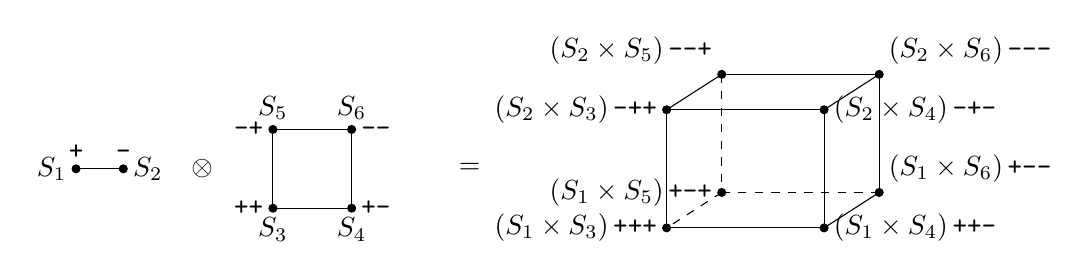
\begin{tikzpicture}
\node[above] at (0,0) {\pp};
\node[left] at (0,0) {$S_1$};
\draw[fill] (0,0) circle [radius=0.05];
\node[above] at (0.6,0) {\mm};
\node[right] at (0.6,0) {$S_2$};
\draw[fill] (0.6,0) circle [radius=0.05];
\draw[-] (0,0) -- (0.6,0);
\node at (1.6,0) {$\otimes$}; 

%%
\node[left] at (2.5,-0.5) {\pp\pp};
\node[below] at (2.5,-0.5) {$S_3$};
\draw[fill] (2.5,-0.5) circle [radius=0.05];
\node[right] at (3.5,-0.5) {\pp\mm};
\node[below] at (3.5,-0.5) {$S_4$};
\draw[fill] (3.5,-0.5) circle [radius=0.05];
\draw[-] (2.5,-0.5) -- (3.5,-0.5);
\draw[-] (2.5,-0.5) -- (2.5,0.5);
\node[left] at (2.5,0.5) {\mm\pp};
\node[above] at (2.5,0.5) {$S_5$};
\draw[fill] (2.5,0.5) circle [radius=0.05];
\node[right] at (3.5,0.5) {\mm\mm};
\node[above] at (3.5,0.5) {$S_6$};
\draw[fill] (3.5,0.5) circle [radius=0.05];
\draw[-] (2.5,0.5) -- (3.5,0.5);
\draw[-] (3.5,-0.5) -- (3.5,0.5);
%% 
\node at (5,0) {$=$};
%% 
\node[left] at (7.5,0.75) {$(S_2 \times S_3)$\,\mm\pp\pp};
\draw[fill] (7.5,0.75) circle [radius=0.05];
\node[right] at (9.5,0.75) {$(S_2 \times S_4)$\,\mm\pp\mm};
\draw[fill] (9.5,0.75) circle [radius=0.05];
\node[above right] at (10.2,1.2) {$(S_2 \times S_6)$\,\mm\mm\mm};
\draw[fill] (10.2,1.2) circle [radius=0.05];
\node[above left] at (8.2,1.2) {$(S_2 \times S_5)$\,\mm\mm\pp};
\draw[fill] (8.2,1.2) circle [radius=0.05];
%%
\node[left] at (7.5,-0.75) {$(S_1 \times S_3)$\,\pp\pp\pp};
\draw[fill] (7.5,-0.75) circle [radius=0.05];
\node[right] at (9.5,-0.75) {$(S_1 \times S_4)$\,\pp\pp\mm};
\draw[fill] (9.5,-0.75) circle [radius=0.05];
\node[above right] at (10.2,-0.3) {$(S_1 \times S_6)$\,\pp\mm\mm};
\draw[fill] (10.2,-0.3) circle [radius=0.05];
\node[left] at (8.2,-0.3) {$(S_1 \times S_5)$\,\pp\mm\pp};
\draw[fill] (8.2,-0.3) circle [radius=0.05];
%%
\draw[-] (7.5,0.75) -- (9.5,0.75);
\draw[-] (9.5,0.75) -- (10.2,1.2);
\draw[-] (10.2,1.2) -- (8.2,1.2);
\draw[-] (8.2,1.2) -- (7.5,0.75);
%%
\draw[-] (7.5,-0.75) -- (9.5,-0.75);
\draw[-] (9.5,-0.75) -- (10.2,-0.3);
\draw[-,dashed] (10.2,-0.3) -- (8.2,-0.3);
\draw[-,dashed] (8.2,-0.3) -- (7.5,-0.75);
%%
\draw[-] (7.5,0.75) -- (7.5,-0.75);
\draw[-] (9.5,0.75) -- (9.5,-0.75);
\draw[-] (10.2,1.2) -- (10.2,-0.3);
\draw[-,dashed] (8.2,1.2) -- (8.2,-0.3);
\end{tikzpicture}
\caption{\label{mult}Example of multiplication of two cubical sets.}
\end{figure*}

This point is made precise in the denotation of types which maps a type of
dimension $n$ to $n$-dimensional cube. We represent such a cube syntactically
as a binary tree of maximum depth $n$ with nodes of the form
$\nodet{\cubt_1}{\cubt_2}$. In such a node, $\cubt_1$ is the positive
subspace and $\cubt_2$ (shaded in gray) is the negative subspace along the
first dimension. Each of these subspaces is itself a cube of a lower
dimension. The $0$-dimensional cubes are the conventional denotation of
first-order types as sets. We use $S$ to denote the denotations of such
types. For example, 1-dimensional cube looks like $\nodet{S_1}{S_2}$ which
intuitively corresponds to the difference $t_1 - t_2$ of the two types whose
denotations are $S_1$ and $S_2$ respectively. A full 2-dimensional cube looks
like $\nodet{(\nodet{S_1}{S_2})}{(\nodet{S_3}{S_4})}$ which intuitively
corresponds to the iterated difference of the appropriate types
$(t_1-t_2)-(t_3-t_4)$ where the product of the successive signs from the
outermost box encodes the sign.

Formally, the denotation of types is as follows:
\[\begin{array}{rcl}
\den{0} &=& \emptyset \\
\den{1} &=& \{ \star \} \\
\den{\tau_1 + \tau_2} &=& \den{\tau_1} \oplus \den{\tau_2} \\
\den{\tau_1 * \tau_2} &=& \den{\tau_1} \otimes \den{\tau_2} \\
\den{- \tau} &=& \ominus \den{\tau} \\
\\
\noalign{\mbox{where:}\hfill}
\\
S_1 \oplus S_2 &=& S_1 \uplus S_2 \\
S \oplus (\nodet{\cubt_1}{\cubt_2}) &=& \nodet{S \oplus \cubt_1}{\cubt_2} \\
(\nodet{\cubt_1}{\cubt_2}) \oplus S &=& \nodet{\cubt_1 \oplus S}{\cubt_2} \\
(\nodet{\cubt_1}{\cubt_2}) \oplus (\nodet{\cubt_3}{\cubt_4}) &=& 
  \nodet{\cubt_1 \oplus \cubt_3}{\cubt_2 \oplus \cubt_4} \\
\\
S_1 \otimes S_2 &=& S_1 \times S_2 \\
S \otimes (\nodet{\cubt_1}{\cubt_2}) &=& 
  \nodet{S \otimes \cubt_1}{S \otimes \cubt_2} \\
(\nodet{\cubt_1}{\cubt_2}) \otimes \cubt &=& 
  \nodet{\cubt_1 \otimes \cubt}{\cubt_2 \otimes \cubt} \\
\\
\ominus~S &=& \nodet{\phantom{S}}{S} \\
\ominus~\nodet{\cubt_1}{\cubt_2} &=& \nodet{\ominus~\cubt_2}{\ominus~\cubt_1} 
\end{array}\]
The type 0 maps to the empty set. The type 1 maps to a singleton set. The sum
of $0$-dimensional types is the disjoint union as expected. For cubes of
higher dimensions, the subspaces are recursively added. Note that the sum of
1-dimensional types reduces to the sum used in the \textbf{Int} construction.
The definition of negation is natural: it recursively swaps the positive and
negative subspaces. The product of 0-dimensional types is the cartesian
product of sets. For cubes of higher-dimensions $n$ and $m$, the result is of
dimension $(n+m)$. The example in Fig.~\ref{mult} illustrates the idea using
the product of 1-dimensional cube (i.e., a line) with a 2-dimensional cube
(i.e., a square). The result is a 3-dimensional cube as illustrated. 

\paragraph*{Note.} 
Our (simple) semantics of types identifies several structurally different
types such as $(1+(1+1))$ and $((1+1)+1)$. In some sense, this is innocent as
the types are isomorphic. However, in the operational semantics discussed in
the next section, we make the computational content of such type isomorphisms
explicit.

\begin{verbatim}
A critical isomorphism that is 
not reflected at all in the semantics
is that 1-1 = 0 

The denotation of 1-1 is a line;
the denotation of 0 is the empty set

[ {*} | {*} ] --> []

Something like the simplification
of Conway games here perhaps?

There are two values of type
1-1

() 
and 
()^-

epsilon should take one and map
to the other because it can
never produce something of type 0

In general, we have several direction
not just left and right like in the
Int construction. In 3D we have
8 directions: +++, ++-, ..., ---
We have an epsilon that 
takes ++- and flips it to --+
and another that flips
+++ to --- and so on

So we should have 8 interpreters
for 3D one for each direction!!!

The ++- interpreter would 
manipulates values like
(v1,v2,v3) and would apply
the normal combinators to v1, v2, 
and the adjoint to v3 and so on.
\end{verbatim}

%%%%%%%%%%%%%%%%%%%%
\subsection{Type Isomorphisms}

\begin{verbatim}
To complete the story we need to 
define morphisms. (More on this below.)
Once we have a notion of morphism we 
can check whether X + 0 is the same
as X etc. i.e., we can check all the 
ring equivalences. 

Ok so what are the morphisms between 
these cubical objects? We know what
they are for 1-dimensional cubes: 
they are the pi combinabors. We also
know what they are for the 2-dimensional 
cubes: a maps (A-B) ==> (C-D) 
is a Pi map between A+D <=> C+B. 
How to generalize this? 

Why is there no trace in the ring 
completion paper??? What are 
the morphisms in that paper?

The ring completion paper produces
a simplicial category.

p. 3 talks about the group cancellation
as subcubes along the diagonal... 

We shouldn't focus on denotations. We want
an operational semantics for pi with 
negatives. The same way that Neel turned
the G construction into code that does
something neat; we want to turn that 
ring completion construction into code
that produces h.o. functions without
losing the multiplicative structure.

Show how to embed a square in 2D into
each of the faces of the 3D cube.

1D into 2D:

(a-b) => (a-b)-(0-0)
(a-b) => (a-0)-(b-0)
(a-b) => (0-b)-(0-a)
(a-b) => (0-0)-(b-a)

\end{verbatim}

%%%%%%%%%%%%%%%%%%%%%%%%%%%%%%%%%%%%%%%%%%%%%%%%%%%%%%%%%%%%%%%%%%%%%%%%%%%%%%
\section{A Reversible Language with Cubical Types} 

We first define values then combinators that manipulate the values to witness
the type isomorphisms.

%%%%%%%%%%%%%%%%%%
\subsection{Values} 

Now that the type structure is defined, we turn our attention to the notion
of values. Intuitively, a value of the $n$-dimensional type $\tau$ is an
element of one of the sets located in one of the corners of the
$n$-dimensional cube denoted by $\tau$. Thus to specify a value, we must
first specify one of the corners of the cube (or equivalently one of the
leaves in the binary tree representation) which can easily be done using a
sequence $p$ of $+$ and $-$ polarities indicating how to navigate the cube in
each successive dimension starting from a fixed origin to reach the desired
corner. We write $v^{p}$ for the value $v$ located at corner $p$ of the cube
associated with its type. We use $\epsilon$ for the empty sequence of
polarities and identify $v$ with $v^\epsilon$. Note that the polarities
doesn't completely specify the type since different types like $(1+(1+1))$
and $((1+1)+1)$ are assigned the same denotation. What the path $p$ specifies
is the \emph{polarity} of the value, or its ``orientation'' in the space
denoted by its type. Formally:
\[\begin{array}{c}
\infer{() : 1}{} \\
\qquad
\infer[\textit{neg}]{v^{\negp{p}} : - \tau}{v^p : \tau} 
\\
\infer[\textit{left}]{(\inl{v})^{p} : \tau_1 + \tau_2}{v^{p} : \tau_1}
\qquad
\infer[\textit{right}]{(\inr{v})^{p} : \tau_1 + \tau_2}{v^{p} : \tau_2} 
\\
\infer[\textit{prod}]{(v_1,v_2)^{p_1 \cdot p_2} : \tau_1 * \tau_2}
      {v_1^{p_1} : \tau_1 & v_2^{p_2} : \tau_2} 
\end{array}\]
The rules \textit{left} and \textit{right} reflect the fact that sums do not
increase the dimension. Note that when $p$ is $\epsilon$, we get the
conventional values for the 0-dimensional sum type. The rule \textit{prod} is
the most involved one: it increases the dimension by \emph{concatenating} the
two dimensions of its arguments. For example, if we pair $v_1^{\pp}$ and
$v_2^{\mm\pp}$ we get $(v_1,v_2)^{\pp\mm\pp}$. (See Fig.~\ref{mult} for the
illustration.) Note again that if both components are 0-dimensional, the pair
remains 0-dimensional and we recover the usual rule for typing values of
product types. The rule \textit{neg} uses the function below which states
that the negation of a value $v$ is the same value $v$ located at the
``opposite'' corner of the cube:
\[\begin{array}{rcl}
\negp{\epsilon} &=& \epsilon \\
\negp{+p} &=& -\negp{p} \\
\negp{-p} &=& +\negp{p}
\end{array}\]

\begin{verbatim}
We only have -
which flips ALL the directions simultaneously.
So from ++-+--+ you can only go to
        --+-++-
What if you wanted to go to
        ++++--+
I think we use the * functor to flip the 
direction we want. 
\end{verbatim}

%%%%%%%%%%%%%%%%%%
\subsection{Combinators: Example} 

Consider the following simple function on 0-dimensional sum types:
\[\begin{array}{rcl}
\textsf{swapP} &\hast& (\tau_1 + \tau_2) \rightarrow (\tau_2 + \tau_1) \\
\textsf{swapP} (\inl{v}) &=& inr{v} \\
\textsf{swapP} (\inr{v}) &=& inl{v}
\end{array}\]
Given our setup, this just works $n$-dimensional types. And so do most of the
$\Pi$ combinators for that matter. Only $\eta$ and $\epsilon$ seem to need
thinking. How and why would $1-1$ which is a 1-dimensional line be the same
as the empty type which is a 0-dimensional thing. And how do we generalize
for arbitrary group identities at higher dimensions. We need a mechanism for
cubes with subspaces that ``cancel'' to map to equivalent smaller subcubes.

%%%%%%%%%%%%%%%%%%
\subsection{$\Pi$ Combinators} 

The terms of $\Pi$ witness type isomorphisms of the form $b \iso b$. They
consist of base isomorphisms, as defined below, and their composition. Each
line of the above table introduces a pair of dual constants\footnote{where
  $\swapp$ and $\swapt$ are self-dual.} that witness the type isomorphism in
the middle.  These are the base (non-reducible) terms of the second,
principal level of $\Pi$. Note how the above has two readings: first as a set
of typing relations for a set of constants. Second, if these axioms are seen
as universally quantified, orientable statements, they also induce
transformations of the (traditional) values. The (categorical or homotopical)
intuition here is that these axioms have computational content because they
witness isomorphisms rather than merely stating an extensional equality.

The isomorphisms are extended to form a congruence relation by adding the
following constructors that witness equivalence and compatible closure:

\begin{table*}[t]
\[\begin{array}{cc}
\begin{array}{rrcll}
\identlp :&  0 + b & \iso & b &: \identrp \\
\swapp :&  b_1 + b_2 & \iso & b_2 + b_1 &: \swapp \\
\assoclp :&  b_1 + (b_2 + b_3) & \iso & (b_1 + b_2) + b_3 &: \assocrp \\
\identlt :&  1 * b & \iso & b &: \identrt \\
\swapt :&  b_1 * b_2 & \iso & b_2 * b_1 &: \swapt \\
\assoclt :&  b_1 * (b_2 * b_3) & \iso & (b_1 * b_2) * b_3 &: \assocrt \\
\distz :&~ 0 * b & \iso & 0 &: \factorz \\
\dist :&~ (b_1 + b_2) * b_3 & \iso & (b_1 * b_3) + (b_2 * b_3)~ &: \factor \\
\eta :&~ 0 & \iso & b + (-b)~ & : \epsilon
\end{array}
& 
\begin{minipage}{0.5\textwidth}
\begin{center} 
\Rule{}
{}
{\jdg{}{}{\idc : b \iso b}}
{}
\qquad\qquad
\Rule{}
{\jdg{}{}{c : b_1 \iso b_2}}
{\jdg{}{}{\symc{c} : b_2 \iso b_1}}
{}
\\ \bigskip
\Rule{}
{\jdg{}{}{c_1 : b_1 \iso b_2} \quad c_2 : b_2 \iso b_3}
{\jdg{}{}{c_1 \fatsemi c_2 : b_1 \iso b_3}}
{}
\\ \bigskip
\Rule{}
{\jdg{}{}{c_1 : b_1 \iso b_2} \quad c_2 : b_3 \iso b_4}
{\jdg{}{}{c_1 \oplus c_2 : b_1 + b_3 \iso b_2 + b_4}}
{}
\\ \bigskip
\Rule{}
{\jdg{}{}{c_1 : b_1 \iso b_2} \quad c_2 : b_3 \iso b_4}
{\jdg{}{}{c_1 \otimes c_2 : b_1 * b_3 \iso b_2 * b_4}}
{}
\end{center}
\end{minipage}
\end{array}\]
\caption{Combinators\label{pi-combinators}}
\end{table*}

It is important to note that ``values'' and ``isomorphisms'' are completely
separate syntactic categories which do not intermix. The semantics of the
language come when these are made to interact at the ``top level'' via
\emph{application}: 
\[\begin{array}{lrcl}
\textit{top level term}, l &::=& c~v
\end{array}\]

%%%%%%%%%%%%%%%%%%%%%%%%%%%%%%%%%%%%%%%%%%%%%%%%%%%%%%%%%%%%%%%%%%%%%%%%%%%%%%
\section{Related Work and Context}

A ton of stuff here. 

%%%%%%%%%%%%%%%%%%%%%%%%%%%%%%%%%%%%%%%%%%%%%%%%%%%%%%%%%%%%%%%%%%%%%%%%%%%%%%
\section{Conclusion}

%%%%%%%%%%%%%%%%%%%%%%%%%%%%%%%%%%%%%%%%%%%%%%%%%%%%%%%%%%%%%%%%%%%%%%%%%%%%%%
\bibliographystyle{abbrvnat}
\softraggedright
\bibliography{cites}

\end{document}



